This section is reserved to explain how microservices can communicate between each other. 
\subsection{Analysing performance}:
When analysing these kind of systems we need to consider the following components:  
\begin{itemize}
    \item The latency; [1]
    \item The complexity; [2]
    \item The scenarios of crashing; [3]
    \item Maintenance; [4]
    \item Scalability; [5]
    \item Stability; [6]
    \item Cost. [7]
\end{itemize}


\subsection{Modes of communication}

There're two modes of communication:
\begin{itemize}
    \item \textbf{Synchronous}: When the requester waits for the response. 
    \item \textbf{Asynchronous}: It's the fire and forget approach. It lauches
    the request and it doesn't wait the response. Eventually it will arrive. 
\end{itemize}

\subsection{Synchronous}

\begin{figure}[h]
\centering
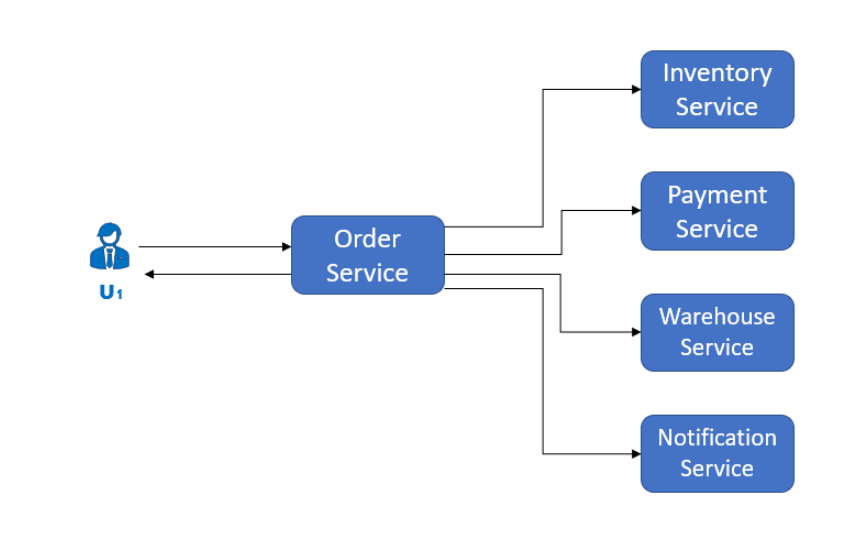
\includegraphics[width=0.8\linewidth]{figures/02_interservice_communication/sync_scenario.png}
\caption{Synchronous scneario}
\label{fig:sync_scenario}
\end{figure}


Consider the occasion where the user \texttt{U1} wants to buy something from Amazon.

The request will be send the \texttt{Order service} that will control the operation.  
First it will ask the \texttt{Inventory Service} if the product is available. In case of yes
it will call the \texttt{Payment service} to perform the payment. Then a request will be sent 
to the \texttt{Warehouse service} and if everything is ok the \texttt{Notification service} 
will send an email message to the user, saying that the product was bought with success or not. 

This is the best scenario that can occur, but what if the \texttt{Payment service} fails? 
We should of course stop the processing. But should we stop it when the \texttt{Notification service} fails? 

\subsubsection{Disadvantages}


The point is that the synchronous approach has some disadvantages: 
\begin{itemize}
    \item The code can become very \textbf{complex}, since we need to handle all the 
    possibilities of failure scenarios. \textit{[3]}
    \item Due to the \textbf{complexity}, it needs high maintenance. \textit{[4]}
    \item It has a very high latency as the user doesn't get notified until a request 
    has been sent and received from the other services. \textit{[1]}
    \item The system is tighly coupled, and any failure will have cascading effects accross the 
    board. \textit{[2]}
\end{itemize}

\subsection{Asynchronous} 

Now let's analyse the same scenario, but with a asynchronous approach.

Creating a full asynchronous approach here would be a big mess! Imagine: we 
send a request to the \texttt{Inventory service}, barely the request is sent we 
start to send another request to the \texttt{Payment service} and so on. But what 
if the payment service is unavailable and it takes a while to send this response?   
Will the user revceive a notification saying that the purchase was done with success 
when it actually wasn't. At this specific part of the code we can use a synchronous
communication and in the warehouse service we can use asynchronous, since we are just
notifying the warehouse about the purchase. 

\subsection{Best of both worlds}

The hybrid approach is what we have just talked about. Is using the asynchronous and 
synchronous approach in one single communication system.   

The mandatory requests are done with synchronous communication and the rest can 
be done with asynchronous: we send an synchronous message to the \texttt{Inventory service}
subtracting the quantity of products to be bought. If the serivice returns an OK response 
we proceed by making a request to the \texttt{Payment service}. If the service respond with an 
OK, than we can make an asynchronous communcation with the \texttt{Warehouse service} and 
\texttt{Notification service}. Otherwise, we just needed to revert the alterations made in 
the \texttt{Inventory}. 

This seems ok by now, but what if the \texttt{Warehouse service} fails? We would loose the details 
of the purchase. That's why in this case we would use the \texttt{Message Queue}. 


\subsection{Message Queue}

The message queues are \hl{highly tolerant to faults}. It has some \hl{Publishers} and 
some \hl{Subscribers}. The publishers publish messages of a certain topic and the subscribers 
reads the message that they're subscribed to. 

\begin{figure}[h]
\centering
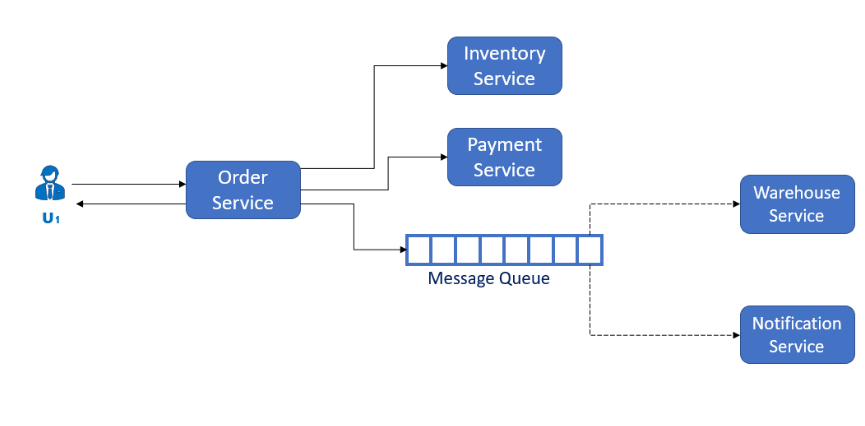
\includegraphics[width=0.8\linewidth]{figures/02_interservice_communication/message_queue.png}
\caption{Message queue}
\label{fig:message_queue}
\end{figure}


Now instead of \texttt{Order service} make a purely asynchronous call to the \texttt{Notificaetion} and 
\texttt{Warehouse} services, it will send a message to the queue. If one of the system is down, the messages
will remain on the queue until the service is back up and ready to receive messages again. 
On this way, none of the data will get lost. 

\subsubsection{Advantages}

\begin{itemize}
    \item \textbf{Increase stability [6]}: Even if a system fails, it will not loose the messages.
    On this way the system becomes more stable. 
    \item \textbf{Enhanced scaling [5]}: When the number of request increases the asynchronous services
    can continue to work in their own pace. Only the synchronous services needs to be scaled by adding 
    more hardware. \textit{My personal opinion is that if the number of requests increase exponentially, 
    then the services that depends on a queue, might also have to be scaled, since the queue can increase 
    to a size, where memory may start to be discarded.}
    \item \textbf{Reduced cost [1] and [7]}: By using queues, not all the services needs to perform 
    synchronous communication. Also, at some level it's not necessary to add extra hardware to the 
    other services. In some aspects this is a win for the wallet. 
    \item \textbf{Reduced complexity [2]}: Since we don't need to handle cascade effects, the code complexity
    is reduced.  

\end{itemize}

\subsection{Building queues}
There're some software that provides this type of communication by queues: 

\begin{itemize}
    \item Kafka
    \item RabbitMQ
    \item ActiveMQ
    \item ZeroMQ
\end{itemize}

